\section{理解视图}
为什么图\ref{fig:xiaoluntaotong}所示的零件图能够唯一也表达\ref{fig:taotonglititu}所示的套筒零件呢,为什么需要两视图呢,一个视图能不能够表达呢,要回答这个问题,需要进一步了解一些与视图相关的知识。
\subsection{视图的概念}
\begin{figure}[htbp]
\centering
\subfloat[斜投影法]{\label{fig:xietouyinfa}
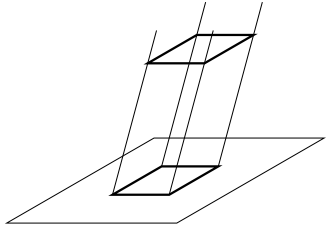
\includegraphics[scale=0.4]{xietoying.png}
}\hspace{30pt}
\subfloat[正投影法]{\label{fig:zhentouyinfa}
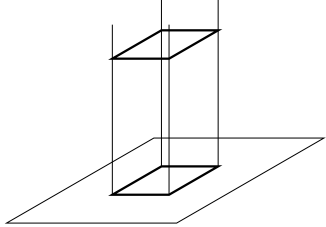
\includegraphics[scale=0.4]{zhengtouying.png}
}
\caption{平行投影法}\label{pingxingtouyin}
\end{figure}

 在图\ref{fig:xiaoluntaotong}所示的套筒零件图中,位于左边的图形称之为主视图,其表达式为全剖视图,关于全剖视图的概念及画法将在后面予以介绍。主视图清晰的表达了套筒零件的长度及内外结构。而位于右边的视图称之为左视图,它清楚地显示套筒零件为回转体类零件。

要理解什么是视图,首先需要了解投影的概念。投影是物体在阳光或灯光下所产生的影子。由于影子只能够表现物体轮廓而不能够表现物体的内部结果,工程实际中将物体内外空间几何元素加以抽象,并用不同的线型进行表示,实现物体内外细节的表达,从而形成的比较完备的、实用的投影方法。投影法分为中心投影法和平行投影法两类。所有投影线都互不平行且汇聚于点的投影法称为中心投影法。中心投影法主要用于绘制效果比较逼真的建筑或产品立体图。图\ref{pingxingtouyin}所示的投影法是平行投影法,从中可以看出其所有的投影线都是相互平行的,其中投影线倾斜于投影面则为斜投影,投影线垂直于投影面则为正投影法。工程中将用正投影法绘制的物体图形称为视图。
\begin{figure}[htbp]
\centering
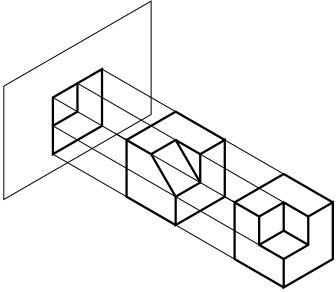
\includegraphics[scale=0.4]{buweiyi.png}
\caption{一个投影面不能确定物体在空间中的形状和位置}\label{fig:singleprojection}
\end{figure}
\subsection{三视图的形成}

\begin{figure}[htbp]
\centering
\subfloat[物体在三面投影中的投影]{\label{fig:threeviewprojection}
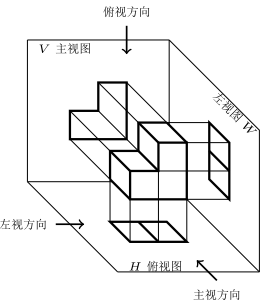
\includegraphics[scale=0.4]{wutisanmiantouying.png}}
\hspace{30pt}
\subfloat[三个投影面的展开]{\label{fig:threeviewzhankai}
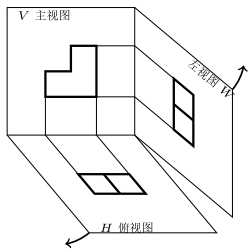
\includegraphics[scale=0.45]{touyingzhankai.png}}


\subfloat[展开后的三视图]{\label{fig:threeview}
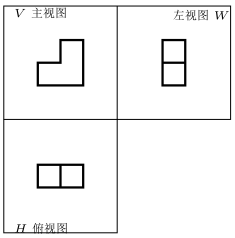
\includegraphics[scale=0.45]{zhankairesult.png}}
\hspace{30pt}
\subfloat[最终三视图]{\label{fig:threeviewguilu}
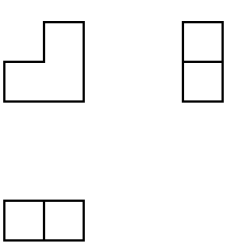
\includegraphics[scale=0.45]{sanshituresult.png}}
\caption{三视图的形成}
\end{figure}
了解完视图的概念后,让们来探讨一个视图能不能够准确地表达出物体的形状这个问题,首先让我们来看一下图\ref{fig:singleprojection}所示的投影。从图\ref{fig:singleprojection}中,我们可以看出不同的形状的物体在同一个视图投影面内具有相同的视图表示。之所以如此,主要是因为仅用一个视图只能反映物体两方向的尺寸,而空间物体需要用长宽高三个方向的尺寸帮能够将其大小形状完整清晰地表达出来。在没有尺寸标注的辅助的情况下,要解决投影只能够表达物体两个尺寸方向的问题,我们需要将物体向多个投影面进行投影,通过多个投影视图来实现物体上下、左右、前后各部分的形状和大小完整表达。在工程零件图中,通常都会使用两个或三个视图来表达一个零件。当然对于简单的轴类零件也经常使用一个视图来表达,对于特别复杂的零件还需要使用更多的辅助视图加以表达。但无论使用多少个视图,三视图是基本的零件图表达方式。下面,我们就来了解一下三视图的形成过程。




为此,我们需要根据国家标准规定,选三个相互垂直的投影面构成图\ref{fig:threeviewprojection}所示的三投影面体系。在三视图投影体系中,正对观察者的投影面称为正平面,用$V$表示。水平放置的投影面称水平面,用$H$表示。侧立的投影面称为侧平面,用$W$表示。将物体放置于三视图投影体系中,将其由前向后投影所得的$V$面视图称为主视;将其由上向下投影所得的$H$面视图称为府视图;将物体由左向右投影所得的$W$面视图称为左视图。最后,按照国家标准,以图\ref{fig:threeviewzhankai}所示方式展开,即以$V$面视图为基准,$H$面绕$V$面与$H$面的交线所形成的$X$轴向下旋转$90^o$;$W$面绕$V$面与$W$面的交线所形成的$Z$轴向右旋转$90^o$,使$V$、$H$、$W$面处于同一个平面内,如图\ref{fig:threeview}所示。展开后的三视图既不需要画边框和投影轴,也不需要标视图名称,如图\ref{fig:threeviewguilu}所示。

\subsection{三视图投影规律}
既然表达一个零件需要多个视图,那么这些视图之间就需要遵循一定规律,才能够准确的表示物体各个组成部分之间的关系。而视图之间所遵循的规律则称之为对应关系。图\ref{fig:threeviewguanxi}标识了三个视图之间的对应关系和视图所能表达的方位。从图中,我们可以得出:主视图反映物体的上下和左右关系,即反映物体的长和高;俯视图反映物体的左右和前后关系,即反映物体的长和宽;左视图反映物体的上下和前后,即反映物体的高和宽。因此,三视图的投影规律为:
\begin{itemize}
\item 主、俯视图长对正;
\item 主、左视图高平齐;
\item 俯、左视图宽相等。
\end{itemize}
\begin{figure}[htbp]
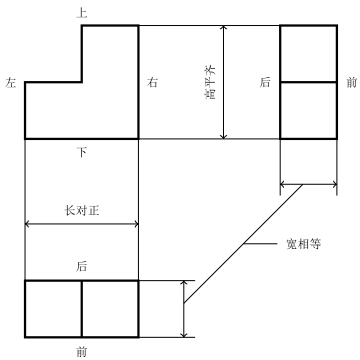
\includegraphics[scale=0.6]{touyingguilu.png}
\caption{三视图投影规律}\label{fig:threeviewguanxi}
\end{figure}
三视图的投影规律不仅适用于物体整体之间的投影,也适用于空间中的点、线面。同时它也是画图和读图的基础规则。由此可知,图\ref{fig:xiaoluntaotong}所示的套筒零件图中,主视图中$\phi 14$尺寸所标法的图线与左视图中的大圆处于同一条水平线上,符合高平齐的对应关系,表达了套筒的外形整体为圆柱体,与此类似,$\phi 8$则表达了套筒的内孔,紧邻大圆的中间圆则表达了倒角。

\endinput